
\chapter{Experimental Results}
\label{chap:exp}

This chapter presents the experiments and the results of the evaluations to the propose robot-camera calibration method as well as to the pose estimation system. In addition to those, an evaluation of the accuracy of the cameras used in this thesis is presented. In order to make such evaluation, the reprojection error, a well understood and known metric in the field of computer vision is used. The reprojection error is an import and crucial step which can determine how accurate the robot-camera calibration can be, for that reason it is performed first, followed by the evaluation of the robot-camera calibration which is essential and determinant step to have a good performance in the pose estimation system, which is the last one to undergo an evaluation process as well.

\section{Robot-Camera Calibration on the Yumi robot}
In order to get an accurate estimation of the robot-camera pose depends on how well the estimation of the intrinsic parameters related to the camera can be. Such estimation of those parameters was accomplished as described in section \ref{pppp}, where those existing algorithms were used for checkerboard detection in both colour and depth data. With those parameter knowing in advance, a reprojection error is calculated for both cameras. 

\subsubsection{Reprojection Error}

The reprojection error is the distance between a pattern keypoint detected in a calibration image, and a corresponding world point projected into the same image. Figure \ref{fig:realopen} and Figure \ref{fig:realros} show the calibration results by analyzing the reprojection error per image for the RealSense camera when OpenCV and camera \textunderscore industrial calibration were used. Figure \ref{fig:astraopen} and Figure \ref{fig:astraros} show the calibration results by analyzing the reprojection error per image for the Astra camera when the OpenCV and camera \textunderscore industrial calibration were used.
%%%%%%%%%%%%%%%%%%%%%%%%%%%%%%%%%%%%%%%%%%
\begin{figure}[!h]
\begin{center}
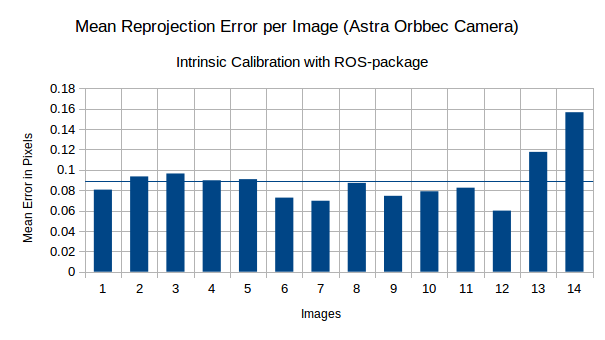
\includegraphics[width=5in, height=3.5in]{figures05/ros_int_cal_astra.png}
\caption{Mean Reprojection Error per image with a ROS method (Astra Orbbec Camera)}%\cite{temp2}}
\label{fig:astraros}
\end{center}
\end{figure}

\begin{figure}[!h]
\begin{center}
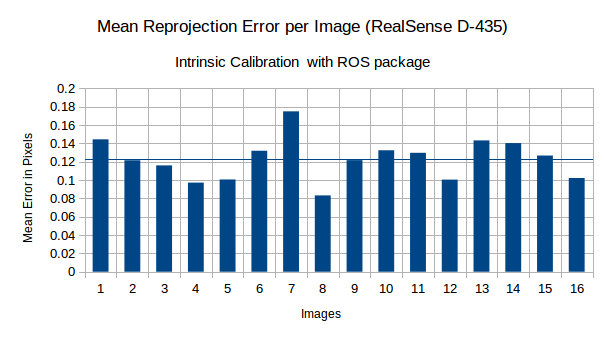
\includegraphics[width=5in, height=3.5in]{figures05/ros_int_cal_real.png}
\caption{Mean Reprojection Error per image with a ROS method (RealSense D-435)}%\cite{temp2}}
\label{fig:realros}
\end{center}
\end{figure}

\begin{figure}[!h]
\begin{center}
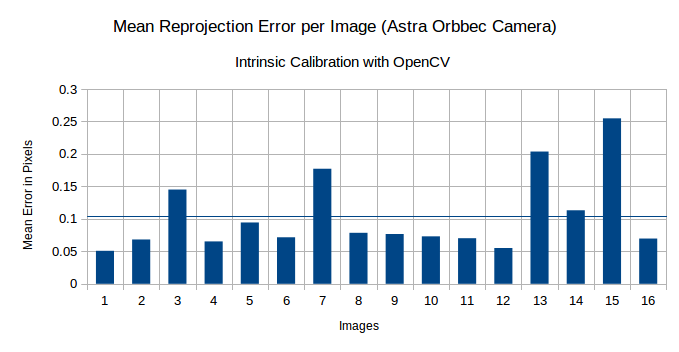
\includegraphics[width=5in, height=3.5in]{figures05/opencv_int_cal_astra.png}
\caption{Mean Reprojection Error per image with a OpenCV method (Astra Orbbec Camera)}%\cite{temp2}}
\label{fig:astraopen}
\end{center}
\end{figure}

\begin{figure}[!h]
\begin{center}
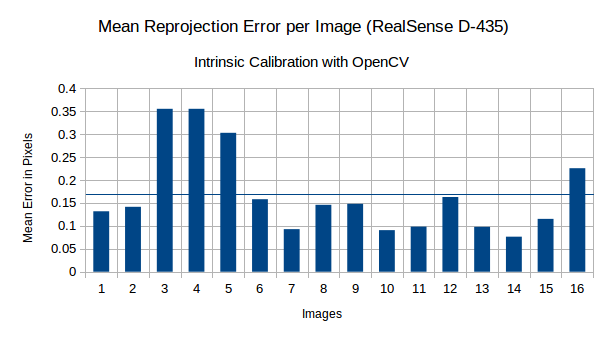
\includegraphics[width=5in, height=3.5in]{figures05/opencv_int_cal_real.png}
\caption{Mean Reprojection Error per image with a OpenCV method (RealSense D-435)}%\cite{temp2}}
\label{fig:realopen}
\end{center}
\end{figure}

To find the average error we calculate the arithmetical mean of the errors calculates for all the calibration images. This should be as close to zero as possible. 
Table \ref{astra1} and Table \ref{real1} show the mean reprojection error for both camera used in this thesis.
As it can be seen in Table \ref{astra1}, the reprojection error for the Astra camera applying both methods, the OpenCV and Astra, are under 0.5 pixels, which it means a good estimation of the intrinsic parameters so far. As to the reprojection errors of its counterpart the RealSense D-435, are shown in the Table \ref{real1}, those values are reasonable and we can determine that both cameras under the same condition were performing good estimates of the internal parameters of the cameras.  The intrinsic parameters are shown in the Appendix \ref{pppppppp}

The reason about using two methods for estimating the intrinsic parameters of both cameras, is the one that we have a clear idea what those values are.  A third method was appied. It was with the use of kalibr, a ros package available in the open source community. The results were not satisfatory, and it is not shown in this thesis. But it is mention as a remark in order to let reader know about its existence for future studies. 

\begin{table}[b]
% increase table row spacing, adjust to taste
\renewcommand{\arraystretch}{1.3}
\caption{Experiment data for internal Astra sensor calibration.}
\label{astra1}
\centering
\begin{tabular}{|c||c|}
\hline
Method & Overall Mean Error\\
\hline
OpenCV &  0.1041954808\\
\hline
ROS &  0.1081118023\\
\hline
\hline
\end{tabular}
\end{table}

\begin{table}[b]
% increase table row spacing, adjust to taste
\renewcommand{\arraystretch}{1.3}
\caption{Experiment data for internal RealSense sensor calibration.}
\label{real1}
\centering
\begin{tabular}{|c||c|}
\hline
Method & Overall Mean Error\\
\hline
OpenCV &  0.1684388411\\
\hline
ROS &  0.122868849\\
\hline
\hline
\end{tabular}
\end{table}

With the evalution of the accuracy of the camera by analizing the reprojection error. The determination and evaluation of the camera pose relative to the robot coordinate follow.

\subsection{Eye-To-Hand Calibration}






\section{Pose Estimation Pipeline}
%%%%%%%%%%%%%%%%%%%%%%%%%%%%%%%%%%%
\iffalse



\begin{itemize}
\item Internal camera calibration where a data collection is requiring.
\item Eye-to-hand calibration where a robot move is requiring. 
\end{itemize}

The propose robot-camera calibration method was successfully performed provided that the checkerboard was detected by the 3D camera to be calibrated.


 Results are divided in two sections, each one requiring an independent set. For an intrinsic calibration, since the extrinsic calibration depends on the known intrinsic parameteres of the camera.  it is not required that the calibration plate be attached to the robot gripper. As to, the extrinsic calibration, the calibration target which is fixed on the customed-made plate is attached to the gripper of the robot.



\subsection{Dataset}

For the performance evaluation, a dataset of scenes was collected. It contains 60 point clouds wich can be classified as:
\begin{itemize}
\item point clouds, captured in a synthetic environment.
\item point clouds, captured in real environment. 
\end{itemize}

\subsection{Metrics}
In this thesis two standard metrics are used in order to evaluate the performance of the pose estimation algorithms.
\begin{itemize}
\item Precision:
\item point clouds, captured in real environment. 
\end{itemize}



\subsection{Testing environment}
The robot-camera calibration method as well as the pose estimation system were implemented in Python within ROS enviornment, making use of highly optimized libraries for 3D point cloud processing and tools. 

\subsection{Hardware}
All tests for which we report the expirements and result have been made using a personal computer Lenovo ThinkPad T430, Intel Core i5-3320 CPU 2.60GHz x 4, 7.8GB RAM, Ubuntu 16.04 64-bit OS
and ROS Kinetic release.

\fi